\begin{tabular}{c}
\centering
\begin{tikzpicture}
\GraphInit[vstyle=Empty]

\Vertex[x=-2, y=1 ]{Y}

\Vertex[x=2,y=0]{Q}

\Vertex[x=-5,y=0]{X}

\Vertex[x=-8,y=-1]{Z}

\Vertex[x=-6,y=-1]{R}

\Vertex[x=-4,y=-1]{A}

\Vertex[x=-2,y=-1]{B}

\Vertex[x=0,y=-1]{C}

\Vertex[x=2,y=-1]{D}

\Vertex[x=4,y=-1]{E}

\Vertex[x=6,y=-1]{F}


\Edges(X,Y,Q) 

\Edges(Z,X,R)

\Edges(A,X,B,Q,C)

\Edges(D,Q,E)

\Edges(E,Q,F)
\end{tikzpicture}
\end{tabular}




%\begin{tikzpicture}[level distance=1.5cm,
%  level 1/.style={sibling distance=1cm},
%  level 2/.style={sibling distance=.5cm}]
%  \node {root}
%    child {node {left}
%    child {node {lleft}}
%    child {node {rleft}}
%    }
%    child {node {right}
%    child {node {lright}}
%    child {node {rright}}
%    };
%
% \node (root) at (0,5) {\begin{tikzpicture}  			\node[circle,draw](){};	\end{tikzpicture} }
%
%	    child {node {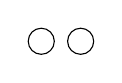
\begin{tikzpicture}\node[circle,draw](n1) at (0,0){};\node[circle,draw](n2) at (0.5,0){};\end{tikzpicture}}
%	    
%      child {node {\begin{tikzpicture}
%  			\node[circle,draw](n5)at (0,0){};\node[circle,draw](n6) at(0.5,0){};\node[circle,draw](n7)at (1,0){};
%			\end{tikzpicture}}}      
%      child {node {\begin{tikzpicture}
%  			\node[circle,draw](n8)at (0,0){};\node[circle,draw](n9) at(0.5,0){};\node[circle,draw](n10)at (1,0){};  			\path[shorten >=1pt, draw, ->] (n8) edge [above] node[font=\tiny] {} (n9);
%  			\end{tikzpicture}}}
%  			} 
%      child {node {\begin{tikzpicture}
%  			\node[circle,draw](n8)at (0,0){};\node[circle,draw](n9) at(0.5,0){};\node[circle,draw](n10)at (1,0){};  			\path[shorten >=1pt, draw, ->] (n9) edge [above] node[font=\tiny] {} (n10);
%  			\end{tikzpicture}}}     
%      child {node {\begin{tikzpicture}
%  			\node[circle,draw](n8)at (0,0){};\node[circle,draw](n9) at(0.5,0){};\node[circle,draw](n10)at (1,0){};  			\path[shorten >=1pt, draw, ->, bend right = 60] (n8) edge [above] node[font=\tiny] {} (n10);
%  			\end{tikzpicture}}}
%      child {node {\begin{tikzpicture}
%  			\node[circle,draw](n8)at (0,0){};\node[circle,draw](n9) at(0.5,0){};\node[circle,draw](n10)at (1,0){};  			\path[shorten >=1pt, draw, ->, bend right = 60] (n8) edge [above] node[font=\tiny] {} (n10);\path[shorten >=1pt, draw, ->] (n8) edge [above] node[font=\tiny] {} (n9);
%  			\end{tikzpicture}}}
%      child {node {\begin{tikzpicture}
%  			\node[circle,draw](n8)at (0,0){};\node[circle,draw](n9) at(0.5,0){};\node[circle,draw](n10)at (1,0){};  			\path[shorten >=1pt, draw, ->, bend right = 60] (n8) edge [above] node[font=\tiny] {} (n10);\path[shorten >=1pt, draw, ->] (n9) edge [above] node[font=\tiny] {} (n10);
%  			\end{tikzpicture}}}
%    child {node{\begin{tikzpicture}
%  			\node[circle,draw](n3)at (0,0){};\node[circle,draw](n4) at(0.5,0){};
%  			\path[shorten >=1pt, draw, ->] (n3) edge [above] node[font=\tiny] {} (n4);
%			\end{tikzpicture}}
%			
%          child {node {\begin{tikzpicture}
%  			\node[circle,draw](n8)at (0,0){};\node[circle,draw](n9) at(0.5,0){};\node[circle,draw](n10)at (1,0){};  			\path[shorten >=1pt, draw, ->, bend right = 60] (n8) edge [above] node[font=\tiny] {} (n10);\path[shorten >=1pt, draw, ->] (n8) edge [above] node[font=\tiny] {} (n9);\path[shorten >=1pt, draw, ->] (n9) edge [above] node[font=\tiny] {} (n10);
%  			\end{tikzpicture}}}
%  			};

%\end{tikzpicture}
